%---------change this every homework
\def\yourid{your name here}
\def\collabs{list your collaborators}
\def\sources{list your sources}
% -----------------------------------------------------
\def\duedate{November 13, 2024 at 11:59p}
\def\pnumber{8}
%-------------------------------------

\RequirePackage[2020-02-02]{latexrelease}
\documentclass[10pt]{article}
\usepackage{dsa2}

\usepackage{tikz-cd}

\begin{document}
\thispagestyle{empty}
\handout

%%%%%%%%%%%%%%%%%%%%%%%%%%%%%%%%%%%%%%%%%%%%%%%%%%%%%%%%

\begin{problem}Arithmetic Optimization\end{problem}
\noindent You are given an arithmetic expression containing $n$ integers and the only operations are additions ($+$) and subtractions ($-$). There are no parenthesis in the expression. For example, the expression might be: $1 + 2 - 3 - 4 - 5 + 6$.

You can change the value of the expression by choosing the best order of operations, for example:
\begin{align*}
 ((((1 + 2) - 3) - 4) - 5) + 6 &= -3 \\
 (((1 + 2) - 3) - 4) - (5 + 6) &= -15\\
 ((1 + 2) - ((3 - 4) - 5)) + 6 &= 15
\end{align*}

Give a {\bf dynamic programming} algorithm that computes the maximum possible value of the expression. You may assume that
the input consists of two arrays: \texttt{nums} which is the list of $n$ integers and \texttt{ops} which is the list of operations (each entry in \texttt{ops} is either \texttt{'+'} or \texttt{'-'}), where \texttt{ops[0]} is the operation between \texttt{nums[0]} and \texttt{nums[1]}. Your answer should include showing expressions from which the min and/or max value is taken, as shown on the slides for the DP solutions that we've covered. Also describe how the intermediate values are stored and where in that memory structure the final answer (maximum possible value) will be. You do not need explain how the optimal ordering can be extracted after the final answer is computed.   \emph{Hint: consider a similar strategy to our algorithm for matrix chaining.}

\solution{
% your solution here
}

  
%%%%%%%%%%%%%%%%%%%%%%%%%%%%%%%%%%%%%%%%%%%%%%%%%%%%%%%%

\begin{problem} More Dominos \end{problem}

In class, we considered the following problem: suppose you are given a rectangular board of size $2$ by $w \geq 1$ (the units here don't matter). You are also given an endless bag of dominoes, each of size $2$ by $1$. Write an algorithm that accepts the integer $w$ as a parameter and returns the total number of unique ways the $2$ by $w$ board can be fully tiled.

Now, for homework, solve the exact same problem as before, except with a board of size $4$ by $w$. Describe your algorithm and state its runtime. For example, if the input given is $w=2$, then the solution is $5$, as shown in the following image (all of the combinations of fully tiled boards of width $w=2$):

{\centering
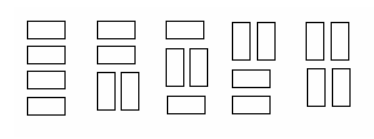
\includegraphics[width=0.5\textwidth]{Dominoes.PNG}
}

\solution{
% your solution here
}


%%%%%%%%%%%%%%%%%%%%%%%%%%%%%%%%%%%%%%%%%%%%%%%%%%%%%%%%



\end{document}
